This section demonstrate the phase-transition phenomenon in model \eqref{eq:model-chisq} with numerical experiments.
The sparsity and signal size of the sparse mean vector are parametrized as in Theorem \ref{thm:chi-squred-strong-boundary}.

\subsection{The strong classification boundary in finite dimensions}

Support set $S$ are estimated using Bonferroni's procedures with FWER decreasing at a rate of $1/\sqrt{\log{p}}$, satisfying the assumptions in Theorem \ref{thm:chi-squred-strong-boundary}.
Experiments were repeated 1000 times under each sparsity-and-signal-size combination.

The results of the numerical experiments are shown in Figure \ref{fig:phase-simulated-chi-squared}.
The numerical results illustrate that the predicted boundaries are not only accurate in high-dimensions ($p=10000$, right panels of Figure \ref{fig:phase-simulated-chi-squared}), but also practically meaningful even at moderate dimensions ($p=100$, left panels of Figure \ref{fig:phase-simulated-chi-squared}).

\begin{figure}
      \centering
      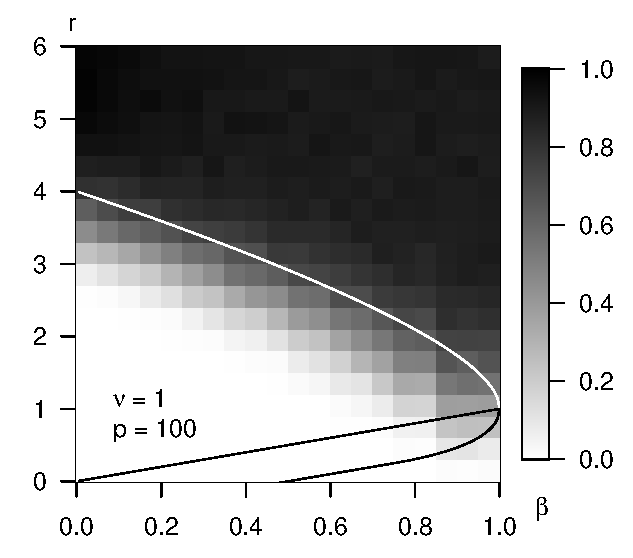
\includegraphics[width=0.32\textwidth]{./sim_strong_boundary/simulated_phase_diagram_chi-squared_nu1_p100.eps}
      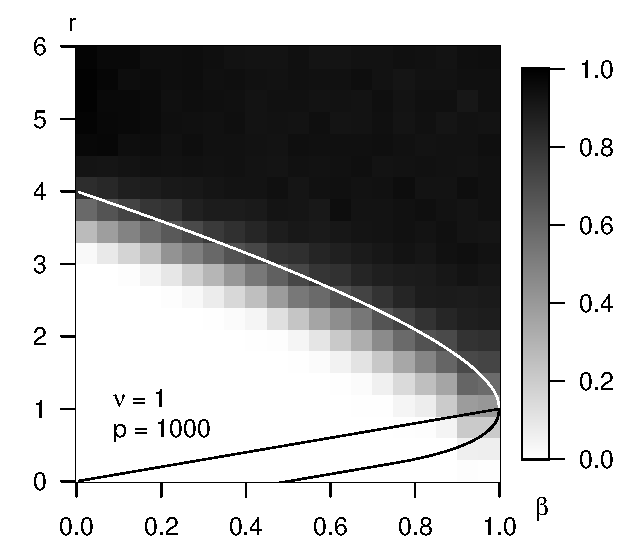
\includegraphics[width=0.32\textwidth]{./sim_strong_boundary/simulated_phase_diagram_chi-squared_nu1_p1000.eps}
      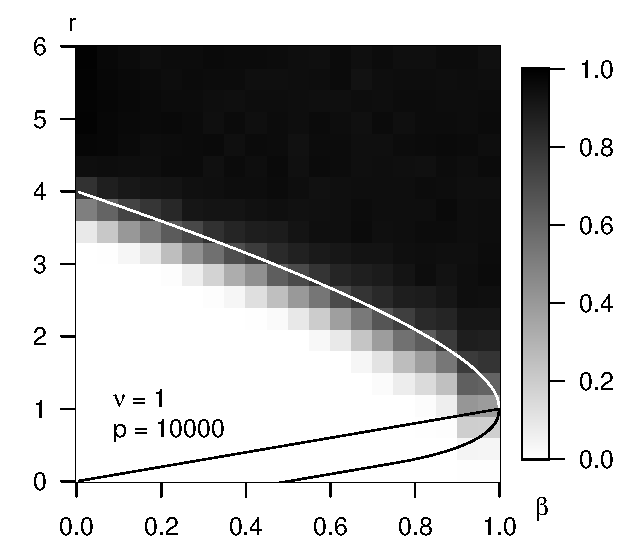
\includegraphics[width=0.32\textwidth]{./sim_strong_boundary/simulated_phase_diagram_chi-squared_nu1_p10000.eps}
      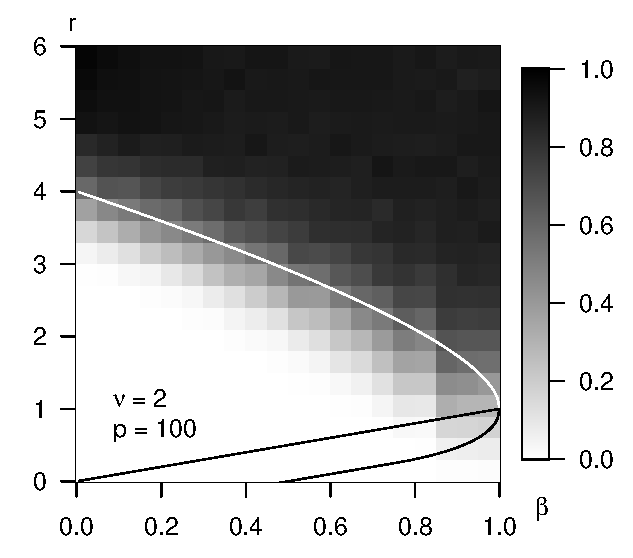
\includegraphics[width=0.32\textwidth]{./sim_strong_boundary/simulated_phase_diagram_chi-squared_nu2_p100.eps}
      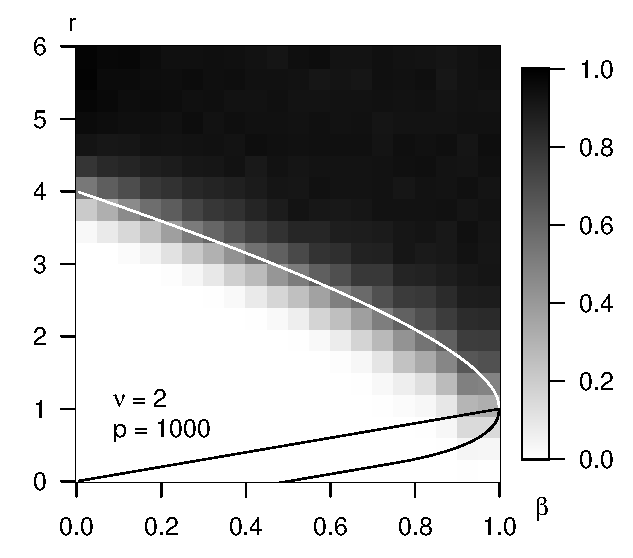
\includegraphics[width=0.32\textwidth]{./sim_strong_boundary/simulated_phase_diagram_chi-squared_nu2_p1000.eps}
      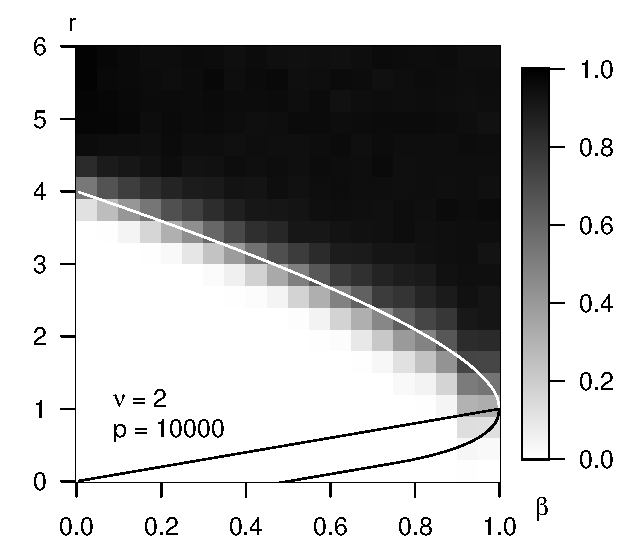
\includegraphics[width=0.32\textwidth]{./sim_strong_boundary/simulated_phase_diagram_chi-squared_nu2_p10000.eps}
      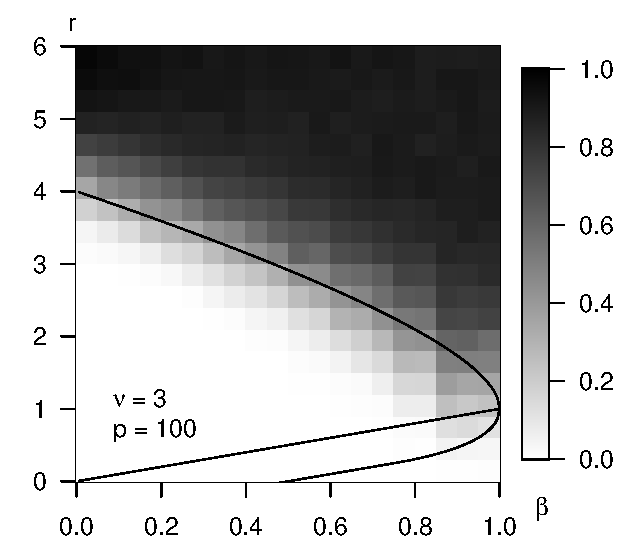
\includegraphics[width=0.32\textwidth]{./sim_strong_boundary/simulated_phase_diagram_chi-squared_nu3_p100.eps}
      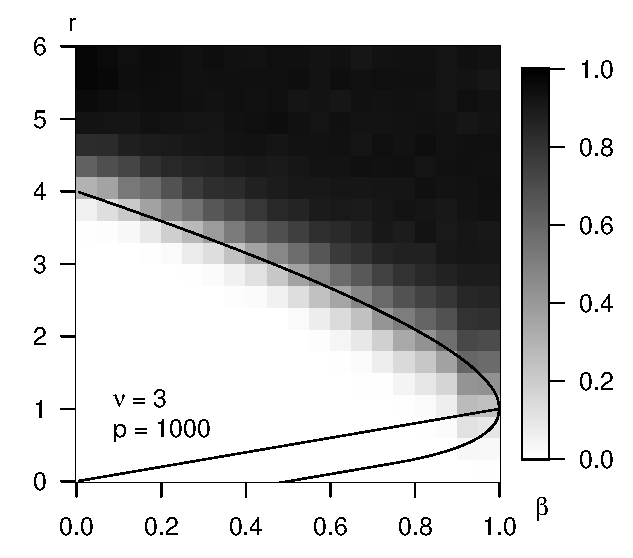
\includegraphics[width=0.32\textwidth]{./sim_strong_boundary/simulated_phase_diagram_chi-squared_nu3_p1000.eps}
      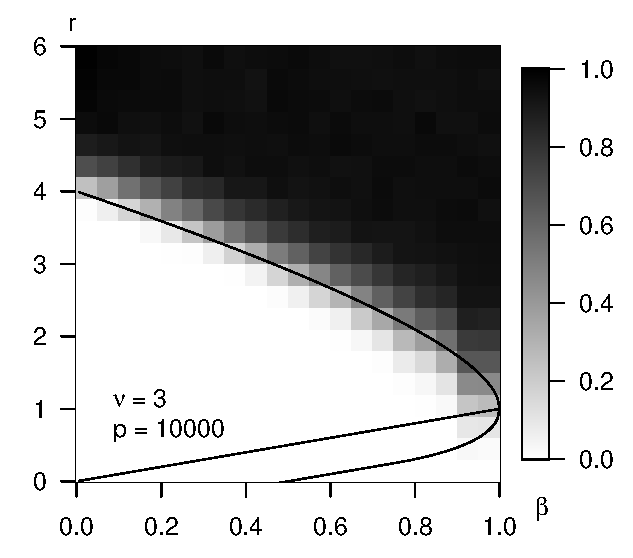
\includegraphics[width=0.32\textwidth]{./sim_strong_boundary/simulated_phase_diagram_chi-squared_nu3_p10000.eps}
      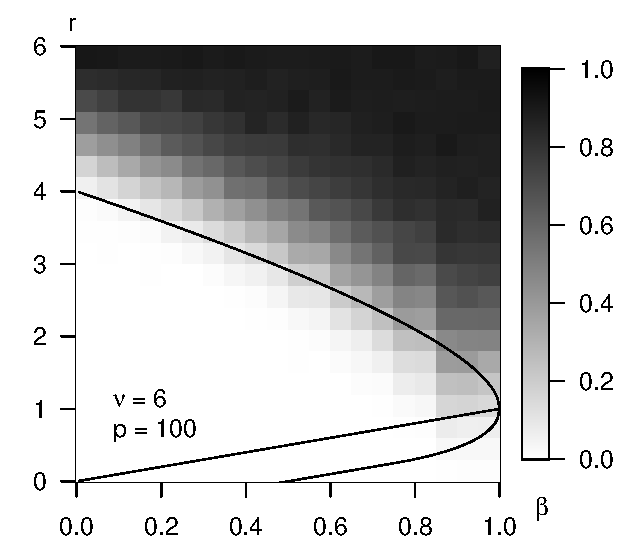
\includegraphics[width=0.32\textwidth]{./sim_strong_boundary/simulated_phase_diagram_chi-squared_nu6_p100.eps}
      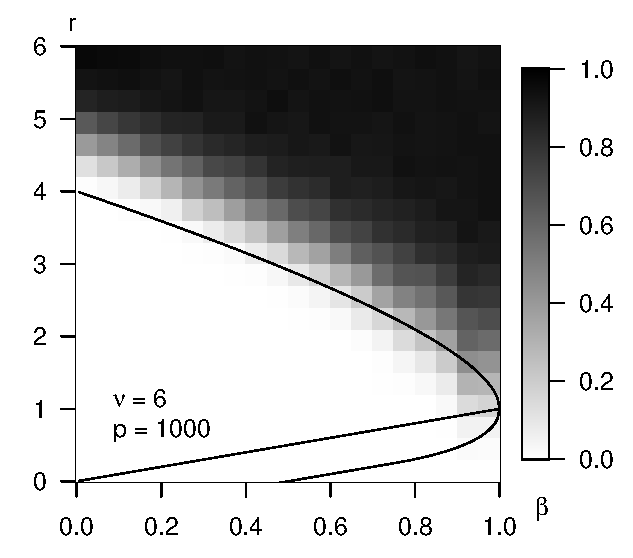
\includegraphics[width=0.32\textwidth]{./sim_strong_boundary/simulated_phase_diagram_chi-squared_nu6_p1000.eps}
      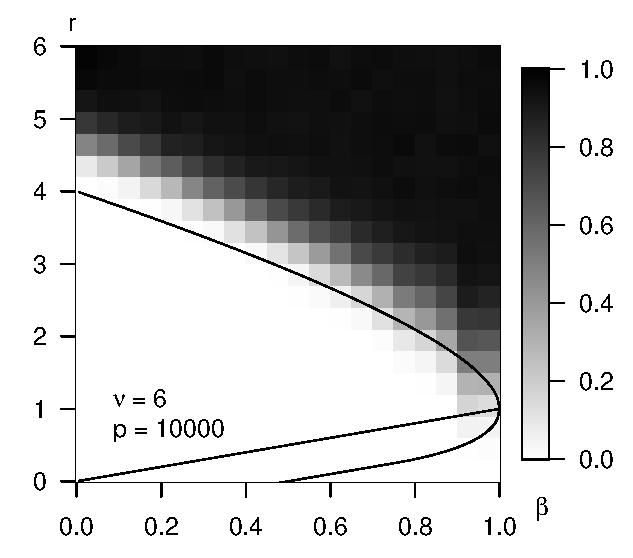
\includegraphics[width=0.32\textwidth]{./sim_strong_boundary/simulated_phase_diagram_chi-squared_nu6_p10000.eps}
      % 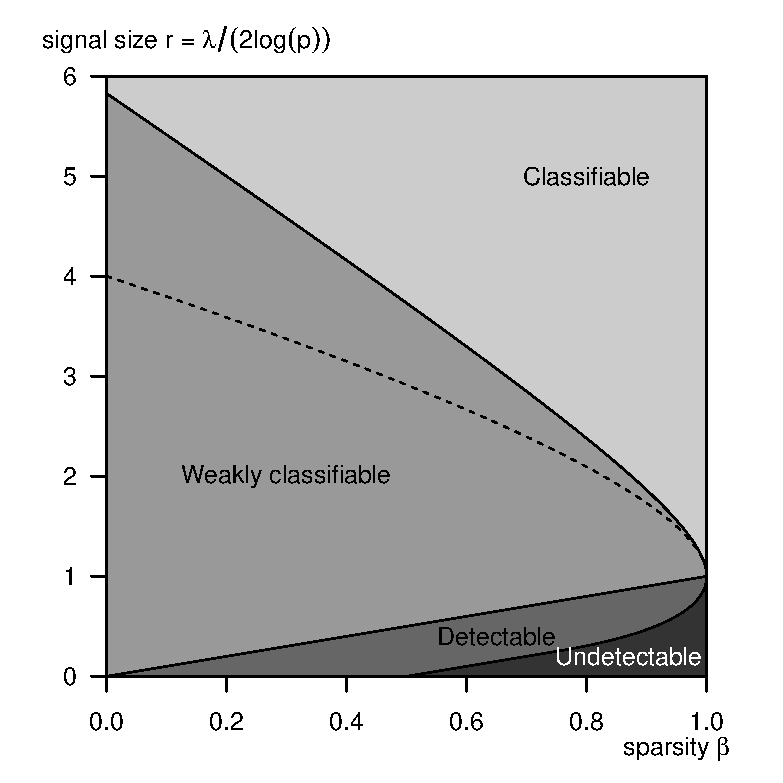
\includegraphics[width=0.35\textwidth]{./phase_diagram_chisquared.eps}
      \caption{The empirical probability of exact support recovery using Bonferroni's procedure in the Chi-squared model \eqref{eq:model-chisq}. 
      We simulate $\nu=1, 2, 3, 6$ (first to last row), at dimensions $p=100, 1000, 10000$ (left to right column), for a grid of sparsity levels $\beta$ and signal sizes $r$.
      The experiments were repeated 1000 times for each sparsity-signal size combination; darker color indicates higher probability of exact support recovery.  
      Numerical results are generally in agreement with the boundaries described in Theorem \ref{thm:chi-squred-strong-boundary}; for large $\nu$'s and finite dimensions, the phase transitions take place somewhat above the predicted boundaries.
      The weak classification boundary (Theorem \ref{thm:chi-squred-weak-boundary}) and the detection boundary (see \citep{donoho2004higher}) are plotted for comparison.} 
      \label{fig:phase-simulated-chi-squared}
\end{figure}



\subsection{The weak classification boundary in finite dimensions}


\begin{figure}
      \centering
      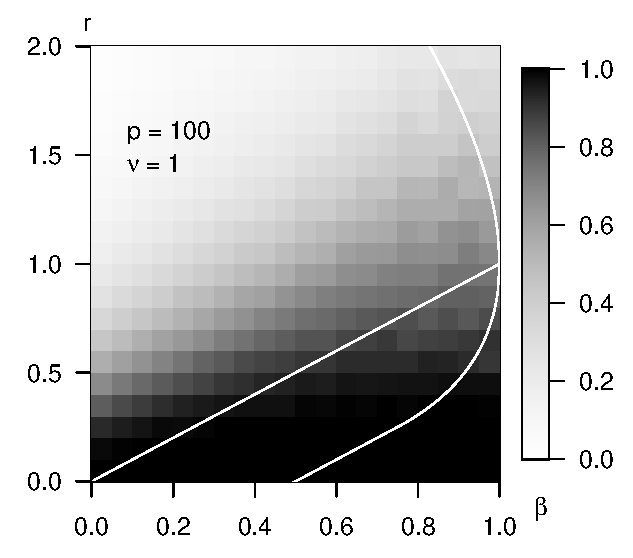
\includegraphics[width=0.32\textwidth]{./sim_weak_boundary/simulated_weak_boundary_chi-squared_nu1_p100.eps}
      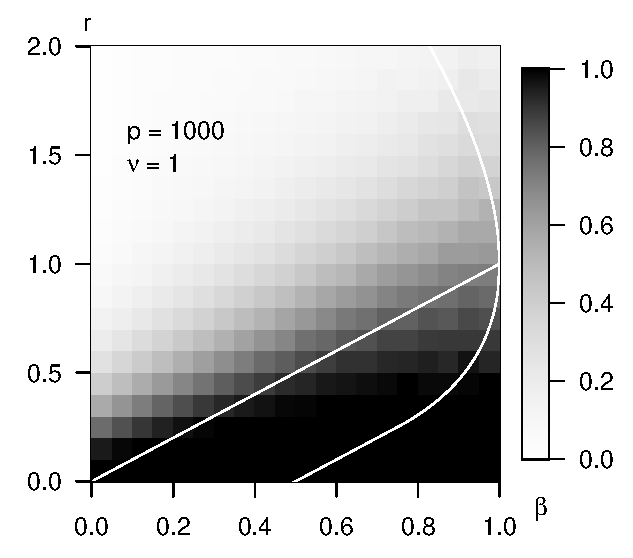
\includegraphics[width=0.32\textwidth]{./sim_weak_boundary/simulated_weak_boundary_chi-squared_nu1_p1000.eps}
      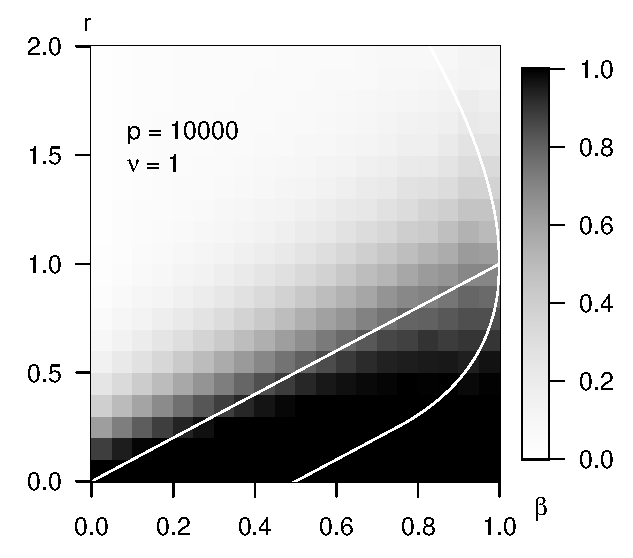
\includegraphics[width=0.32\textwidth]{./sim_weak_boundary/simulated_weak_boundary_chi-squared_nu1_p10000.eps}
      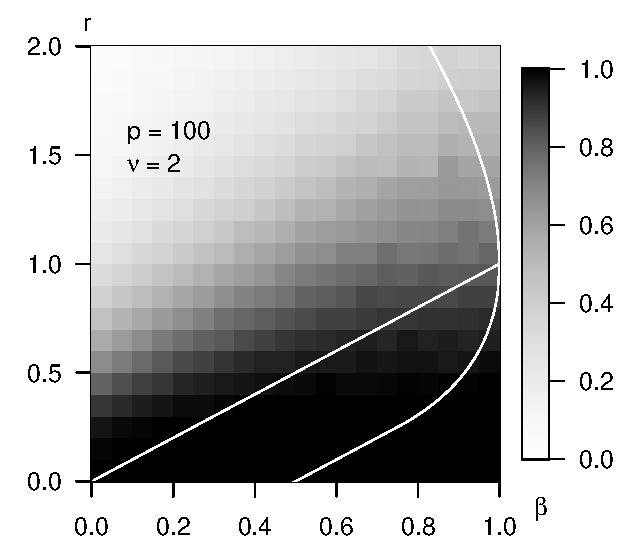
\includegraphics[width=0.32\textwidth]{./sim_weak_boundary/simulated_weak_boundary_chi-squared_nu2_p100.eps}
      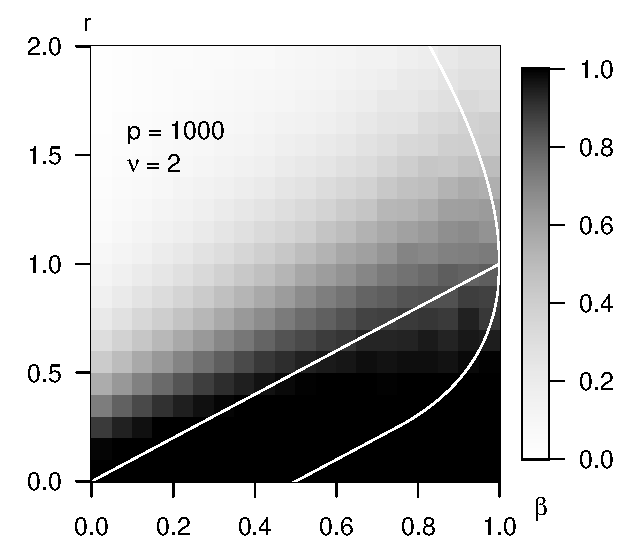
\includegraphics[width=0.32\textwidth]{./sim_weak_boundary/simulated_weak_boundary_chi-squared_nu2_p1000.eps}
      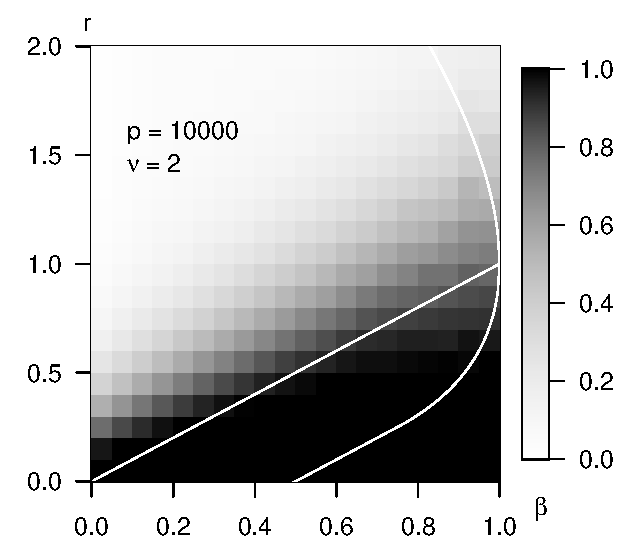
\includegraphics[width=0.32\textwidth]{./sim_weak_boundary/simulated_weak_boundary_chi-squared_nu2_p10000.eps}
      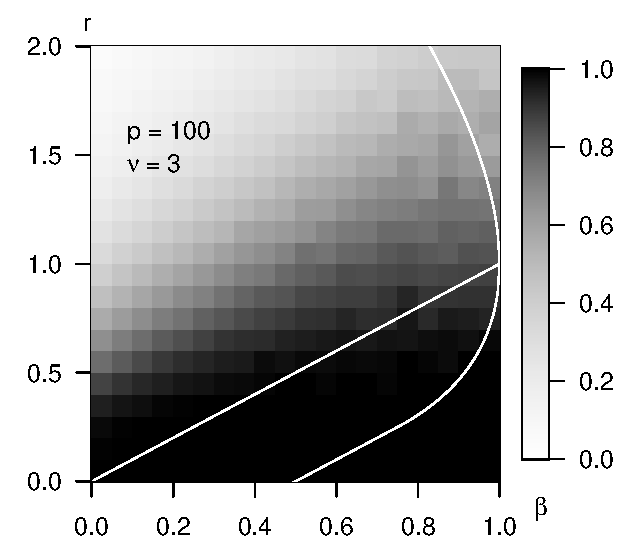
\includegraphics[width=0.32\textwidth]{./sim_weak_boundary/simulated_weak_boundary_chi-squared_nu3_p100.eps}
      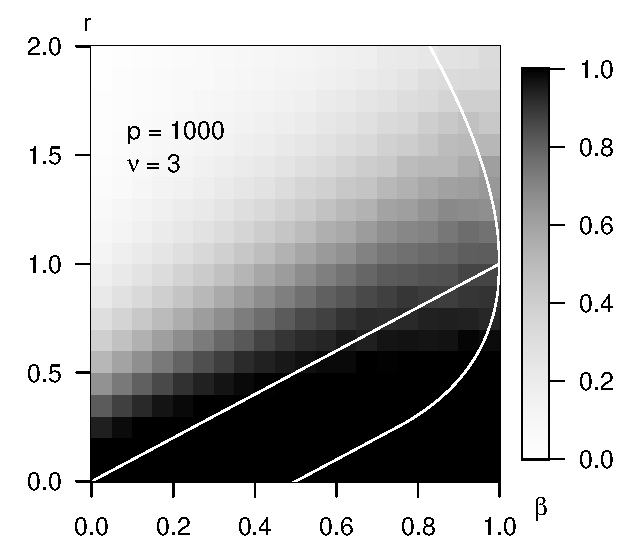
\includegraphics[width=0.32\textwidth]{./sim_weak_boundary/simulated_weak_boundary_chi-squared_nu3_p1000.eps}
      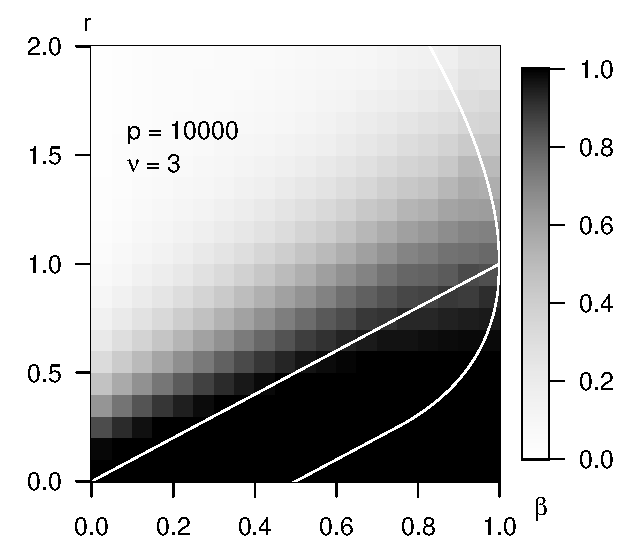
\includegraphics[width=0.32\textwidth]{./sim_weak_boundary/simulated_weak_boundary_chi-squared_nu3_p10000.eps}
      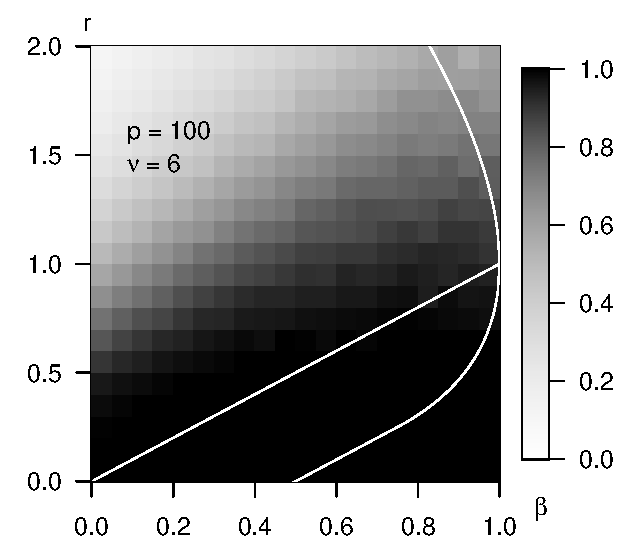
\includegraphics[width=0.32\textwidth]{./sim_weak_boundary/simulated_weak_boundary_chi-squared_nu6_p100.eps}
      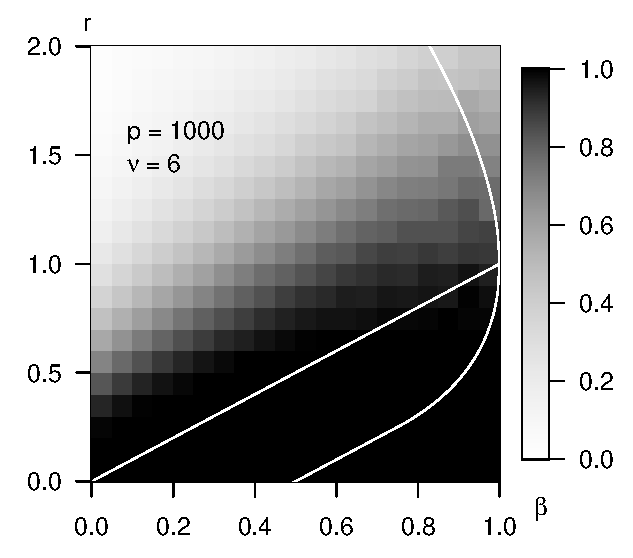
\includegraphics[width=0.32\textwidth]{./sim_weak_boundary/simulated_weak_boundary_chi-squared_nu6_p1000.eps}
      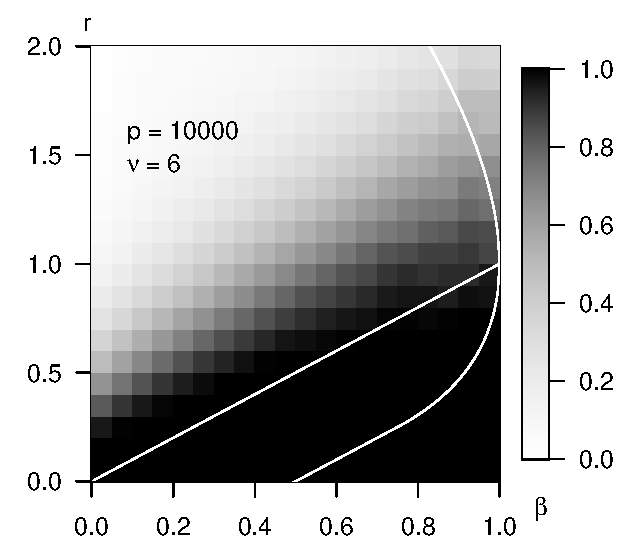
\includegraphics[width=0.32\textwidth]{./sim_weak_boundary/simulated_weak_boundary_chi-squared_nu6_p10000.eps}
      % 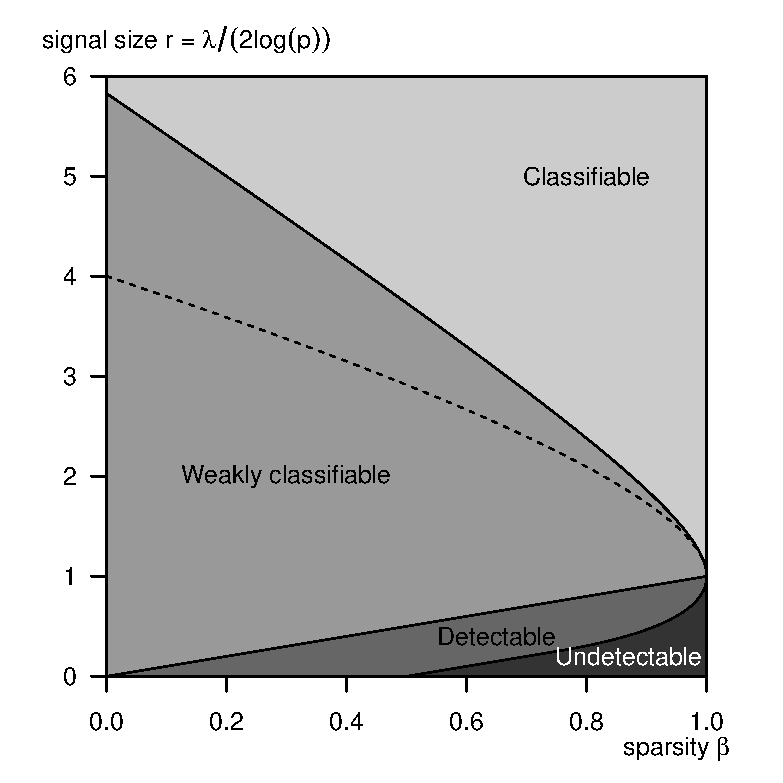
\includegraphics[width=0.35\textwidth]{./phase_diagram_chisquared.eps}
      \caption{The estimated risk of approximate support recovery $\mathrm{risk}^{\mathrm{A}}$ (see \eqref{eq:risk-approximate}) of the Benjamini-Hochberg procedure in the Chi-squared model \eqref{eq:model-chisq}. 
      We simulate $\nu=1, 2, 3, 6$ (first to last row), at dimensions $p=100, 1000, 10000$ (left to right column), for a grid of sparsity levels $\beta$ and signal sizes $r$.
      The experiments were repeated 1000 times for each sparsity-signal size combination; darker color indicates higher larger $\mathrm{risk}^{\mathrm{A}}$. 
      Numerical results are generally in agreement with the boundaries described in Theorem \ref{thm:chi-squred-weak-boundary}; for large $\nu$'s and finite dimensions, the phase transitions take place somewhat above the predicted boundaries.
      The strong classification boundary (Theorem \ref{thm:chi-squred-strong-boundary}) and the detection boundary (see \citep{donoho2004higher}) are plotted for comparison.} 
      \label{fig:phase-simulated-chi-squared-weak-boundary}
\end{figure}

\subsection{Phase transitions of reported findings from GWAS}